\chapter{序論}
\label{chap:introduction}

本章では,本研究の背景と本論文の構成について述べる.

\newpage

\section{背景}

現在,知りたい情報を探す方法としてインターネットは多く利用されている.特に Web ブラウザでの情報検索は社会生活を送る中で必要不可欠である.

情報検索において,一般的には古い情報よりも新しい情報の方が価値が高い.しかし Web 検索結果一覧の各情報は実世界に存在する紙やインクのように時間経過による外見的な劣化がないため,情報の鮮度を直感的に判断するのは難しい.

\begin{figure}[htbp]
  \begin{minipage}{0.3\hsize}
    \begin{center}
      \fbox{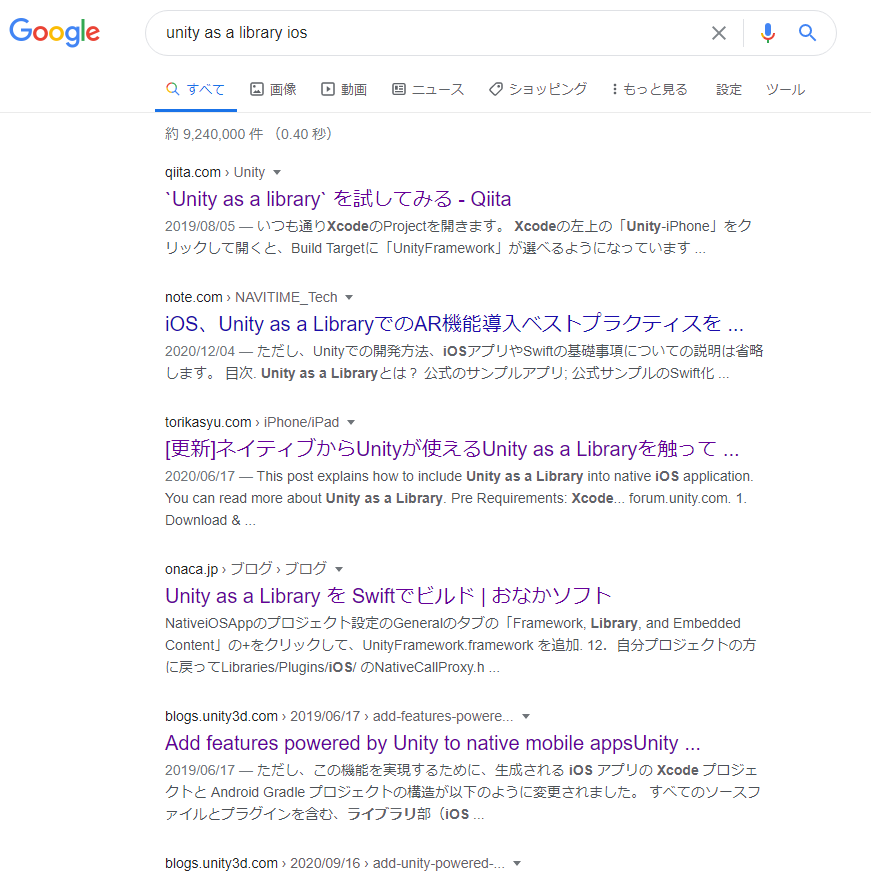
\includegraphics[width=60mm]{images/search-google.png}}
    \end{center}
    \caption{Google\footnote{https://www.google.com/} の検索結果一覧画面}
  \end{minipage}
  \begin{minipage}{0.3\hsize}
    \begin{center}
      \fbox{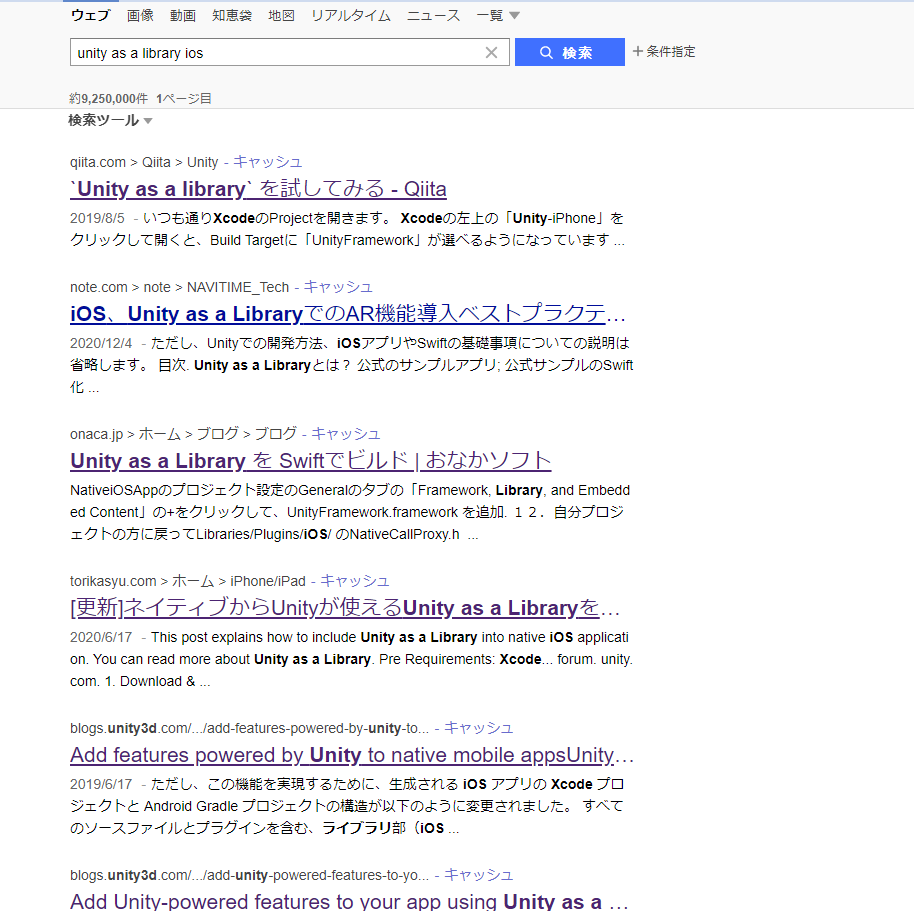
\includegraphics[width=60mm]{images/search-yahoo.png}}
    \end{center}
    \caption{Yahoo!\footnote{https://www.yahoo.co.jp/} の検索結果一覧画面}
  \end{minipage}
  \begin{minipage}{0.3\hsize}
    \begin{center}
      \fbox{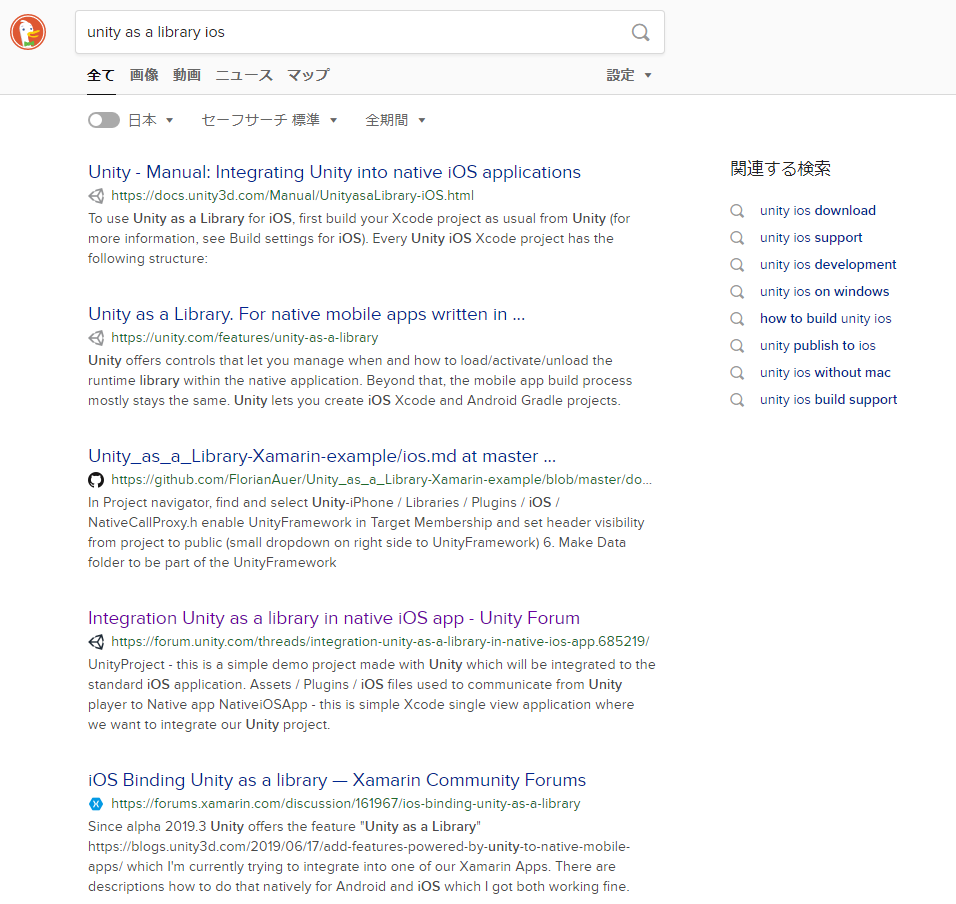
\includegraphics[width=60mm]{images/search-ddg.png}}
    \end{center}
    \caption{DuckDuckGo\footnote{https://duckduckgo.com/} の検索結果一覧画面}
  \end{minipage}
\end{figure}

そこで本来外見的な劣化のない各情報に,時間経過による表示の変化を与える.これにより情報の鮮度を直感的に認識できるようになり,効率的に Web 検索による情報収集を行うことができると考えた.

また,松下\cite{tecvisinfo}らの解説によれば,増え続ける Web ページの数に対して,ページランキングの精度に限界があるため,情報可視化システムにかかる期待は今後も大きくなると予測される.

近似研究として廃れるリンク\cite{dyinglink}がある.こちらはリンク先のページの鮮度に応じてリンクを廃れさせる情報視覚化システムである.

しかし,リンクのみへの適用であるため鮮度の表現方法に改善の余地があると考えた.

\section{本研究の目的}

ブラウザにおける検索結果一覧画面を拡張することで,ユーザがより直感的に情報の鮮度を認識できるようにすることが本研究の目的である.

\section{本文書の構成}

第\ref{chap:introduction}章では本研究における背景と目的について述べた.

第\ref{chap:verification}章では実際に視覚化システムを開発する前に様々な視覚化の方法を試し評価した.

第\ref{chap:implementation}章で開発したシステムの実装に関して述べ,第\ref{chap:discussion}章では実際に利用して得られた評価や今後の展望について述べた.

第\ref{chap:survey}章では本研究と関連のある研究事例を紹介している.第\ref{chap:conclusion}章では本研究を総括して結論を述べる.
